\RequirePackage{xcolor}
\documentclass[a0]{sciposter} % mayor hoja estandar
\usepackage{multicol,subfig,amsmath}
\usepackage{graphicx,url,hyperref,doi}
\usepackage[spanish]{babel}   
\usepackage[utf8]{inputenc}
\usepackage[sort&compress,numbers]{natbib}
\usepackage{tikz}
\usepackage{adjustbox}

\usepackage{dingbat}



\tikzstyle{elem} = [draw, rectangle, thick, minimum height=2em, minimum width=2em]
\tikzstyle{line} = [draw, thick, -stealth, shorten >=1pt]

\setlength{\parskip}{3pt}
\renewcommand{\arraystretch}{1.5}

\title{Modelado y visualización de relaciones entre contaminantes del aire y salud pública}
\author{Selene Berenice Prado Prado$^\dagger$, Satu Elisa Schaeffer$^\ast$}
\institute {$^\dagger$ Ingeniería en Tecnología de Software, $^\ast$ Posgrado en Ingeniería de Sistemas}
\email{$^\dagger$selene.pradopr@uanl.edu.mx, $^\ast$elisa.schaeffer@uanl.edu.mx}
\leftlogo[1]{uanl.png} 
\rightlogo[1]{fime.png}

\begin{document}


\maketitle

\begin{abstract}
El objetivo de la investigación es generar modelos que permitan visualizar relaciones entre contaminantes atmosféricos y salud pública. El tener un modelo que permita visualizar relaciones entre contaminantes atmosféricos y salud pública que sea utilizado con datos confiables y verídicos pueden ayudar a entender el impacto que tiene el aumento del nivel de contaminantes atmosféricos.  En la investigación se exploran diversas maneras de visualizar la información y se generan modelos que permiten analizar relaciones entre niveles de contaminantes y CIE. 
%Las visualizaciones generadas son series de tiempo y gráficos de radar, y modelos de regresión lineal y de regresión lineal múltiple.
\end{abstract}

\begin{multicols}{3} 

\section{Introducción}
La tarea en el presente proyecto es utilizar modelos para visualizar las relaciones entre los contaminantes del aire y salud pública. Para la realización de los experimentos se tienen datos de ingresos hospitalarios provenientes de la base de datos de la Secretaría de Salud del Gobierno de México \cite{f1}. También se tienen registros de los niveles de algunos contaminantes del aire presentes en el área metropolitana de Monterrey, capturados por las estaciones de monitoreo pertenecientes al Sistema Integral de Monitoreo Ambiental (SIMA) \cite{f2} mostradas en la figura \ref{estaciones}.
\begin{figure}[h!]
\setcounter{figure}{0} % por culpa de sciposter
\captionsetup{type=figure} % por culpa de sciposter
\begin{center}
   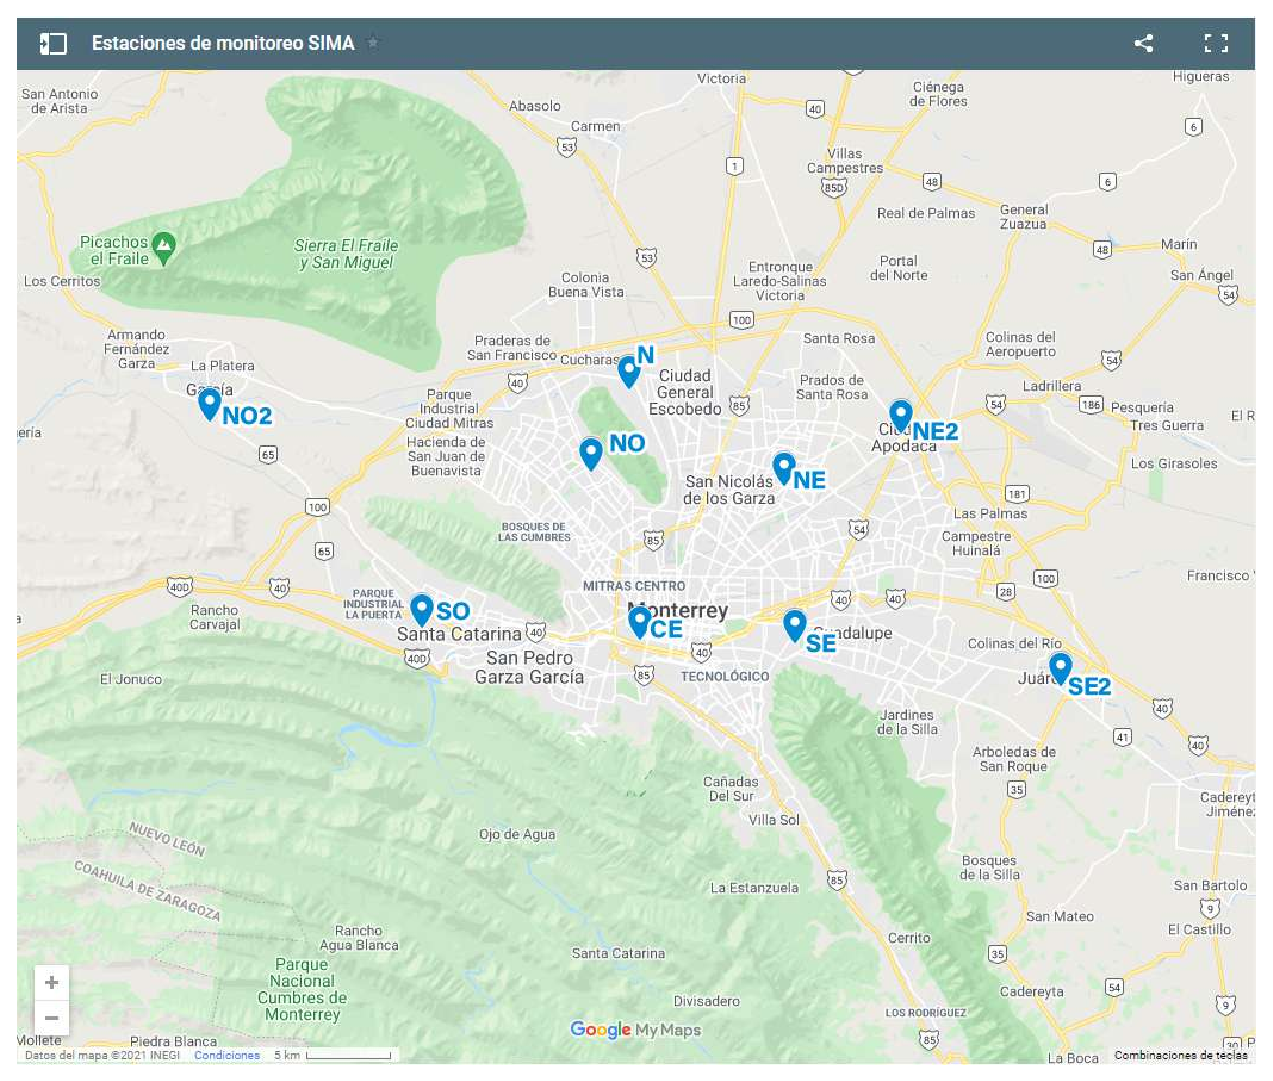
\includegraphics[trim=50 50 50 50,clip,width=0.9\textwidth]{mapa_estaciones.eps}
   \end{center}
    \caption{Localización de las estaciones de monitoreo de la calidad del aire.}
    \label{estaciones}
\end{figure}

\section{Antecedentes}
En Nuevo León, México, las operaciones de la Red Automática de Monitoreo Atmosférico iniciaron en 1993 con cinco estaciones fijas \citep{r4}. Como se muestra en la figura \ref{estaciones}, actualmente se cuenta con nueve estaciones que monitorean los siguientes contaminantes: monóxido de carbono (CO), dióxido de azufre (SO$_2$), óxidos de nitrógeno (NO$_x$), ozono (O$_3$), partículas de tamaño menor a 10 micrómetros (PM10) y partículas de tamaño menor a 2.5 micrómetros (PM2.5).

Algunos conceptos importantes a definir para este proyecto son:
\begin{itemize}
	\item Serie de tiempo: Conjunto de observaciones tomadas en un tiempo $t$ determinado. Relacionan estadísticamente los cambios temporales en la repercusión de cambios en la concentración de un contaminante en la población.
	\item Clasificación Internacional de Enfermedades (CIE): Instrumento estadístico y sanitario para identificar enfermedades agrupándolas en epidémicas, generales, locales ordenadas por origen geográfico, trastornos del desarrollo y lesiones.
	\item Regresión lineal: Metodología inferencial supervisada que busca predecir valores $y$ dado un vector de variables de entrada $t$ por medio del ajuste de coeficientes $w$.
	\item Regresión lineal múltiple: Modelo complemento de la regresión lineal simple, el cual tiene dos o más variables independientes $k$ que pueden influir en una variable dependiente $y$.
\end{itemize}

\section{Estado de arte}
Se estudia literatura reciente relacionada con el presente trabajo con el objetivo de revisar distintos métodos para resolver el problema planteado y, además, revisar implementaciones similares para resolver problemas distintos. Lo anterior tiene la finalidad de comparar los trabajos revisados e identificar áreas de oportunidad en ellos.

\begin{table}[hbt!]
\centering
\captionsetup{type=table}
\setcounter{table}{0}
\caption{Comparación de trabajos frente al desarrollado, donde  \checkmark indica que cumple con esta característica y  $\times$ no cumple con esta característica.}
\begin{tabular}{|l|c|c|c|c|c|}
\hline
Trabajo & \rotatebox[origin=c]{90}{ Modelos de regresión lineal } & \rotatebox[origin=c]{90}{ Modelos de predicción } & \rotatebox[origin=c]{90}{ Evaluación de modelos } & \rotatebox[origin=c]{90}{ Estudio de contaminantes del aire } & \rotatebox[origin=c]{90}{ Estudio de problemas de salud }\\
	\hline
    \citet{r12} & \checkmark & $\times$ & $\times$ & \checkmark & \checkmark\\
    \hline
    \citet{r13} &  $\times$ & \checkmark & \checkmark & \checkmark & $\times$\\
    \hline
    \citet{r14} & \checkmark & \checkmark & $\times$ & \checkmark & \checkmark\\
    \hline
    \citet{r15} & \checkmark & \checkmark & $\times$ & \checkmark & \checkmark\\
	\hline    
    \citet{r16}& \checkmark & $\times$ & $\times$ & \checkmark & \checkmark\\
	\hline    
    \citet{r17} & $\times$ & \checkmark & \checkmark & \checkmark & \checkmark\\
	\hline    
    \citet{r18} & $\times$  & $\times$ & $\times$ & \checkmark & \checkmark\\
	\hline    
    \citet{r19} & \checkmark & \checkmark & $\times$ & \checkmark & \checkmark\\
	\hline    
    \citet{r20} &  \checkmark & \checkmark & $\times$ & \checkmark & \checkmark\\
	\hline    
    El presente trabajo & \checkmark & \checkmark & \checkmark & \checkmark & \checkmark\\
    \hline
\end{tabular}
\label{tab:Comparación de trabajos frente al desarrollado}
\end{table}

\section{Solución propuesta}
La solución propuesta se compone de cuatro fases: recolección de datos, selección y agrupación de datos, visualización de la evolución de las variables e implementación de modelos.
Los tipos de visualizaciones generadas son: series de tiempo y gráficos de radar (ejemplos en las figuras \ref{serie_de_tiempo_2017_PM10} y \ref{grafico_de_telaraña}). Los tipos de modelos generados son: modelos de regresión lineal y modelos de regresión lineal múltiple.
	
\begin{figure}[h!]
\setcounter{figure}{1} % por culpa de sciposter
\captionsetup{type=figure} % por culpa de sciposter
\begin{center}
   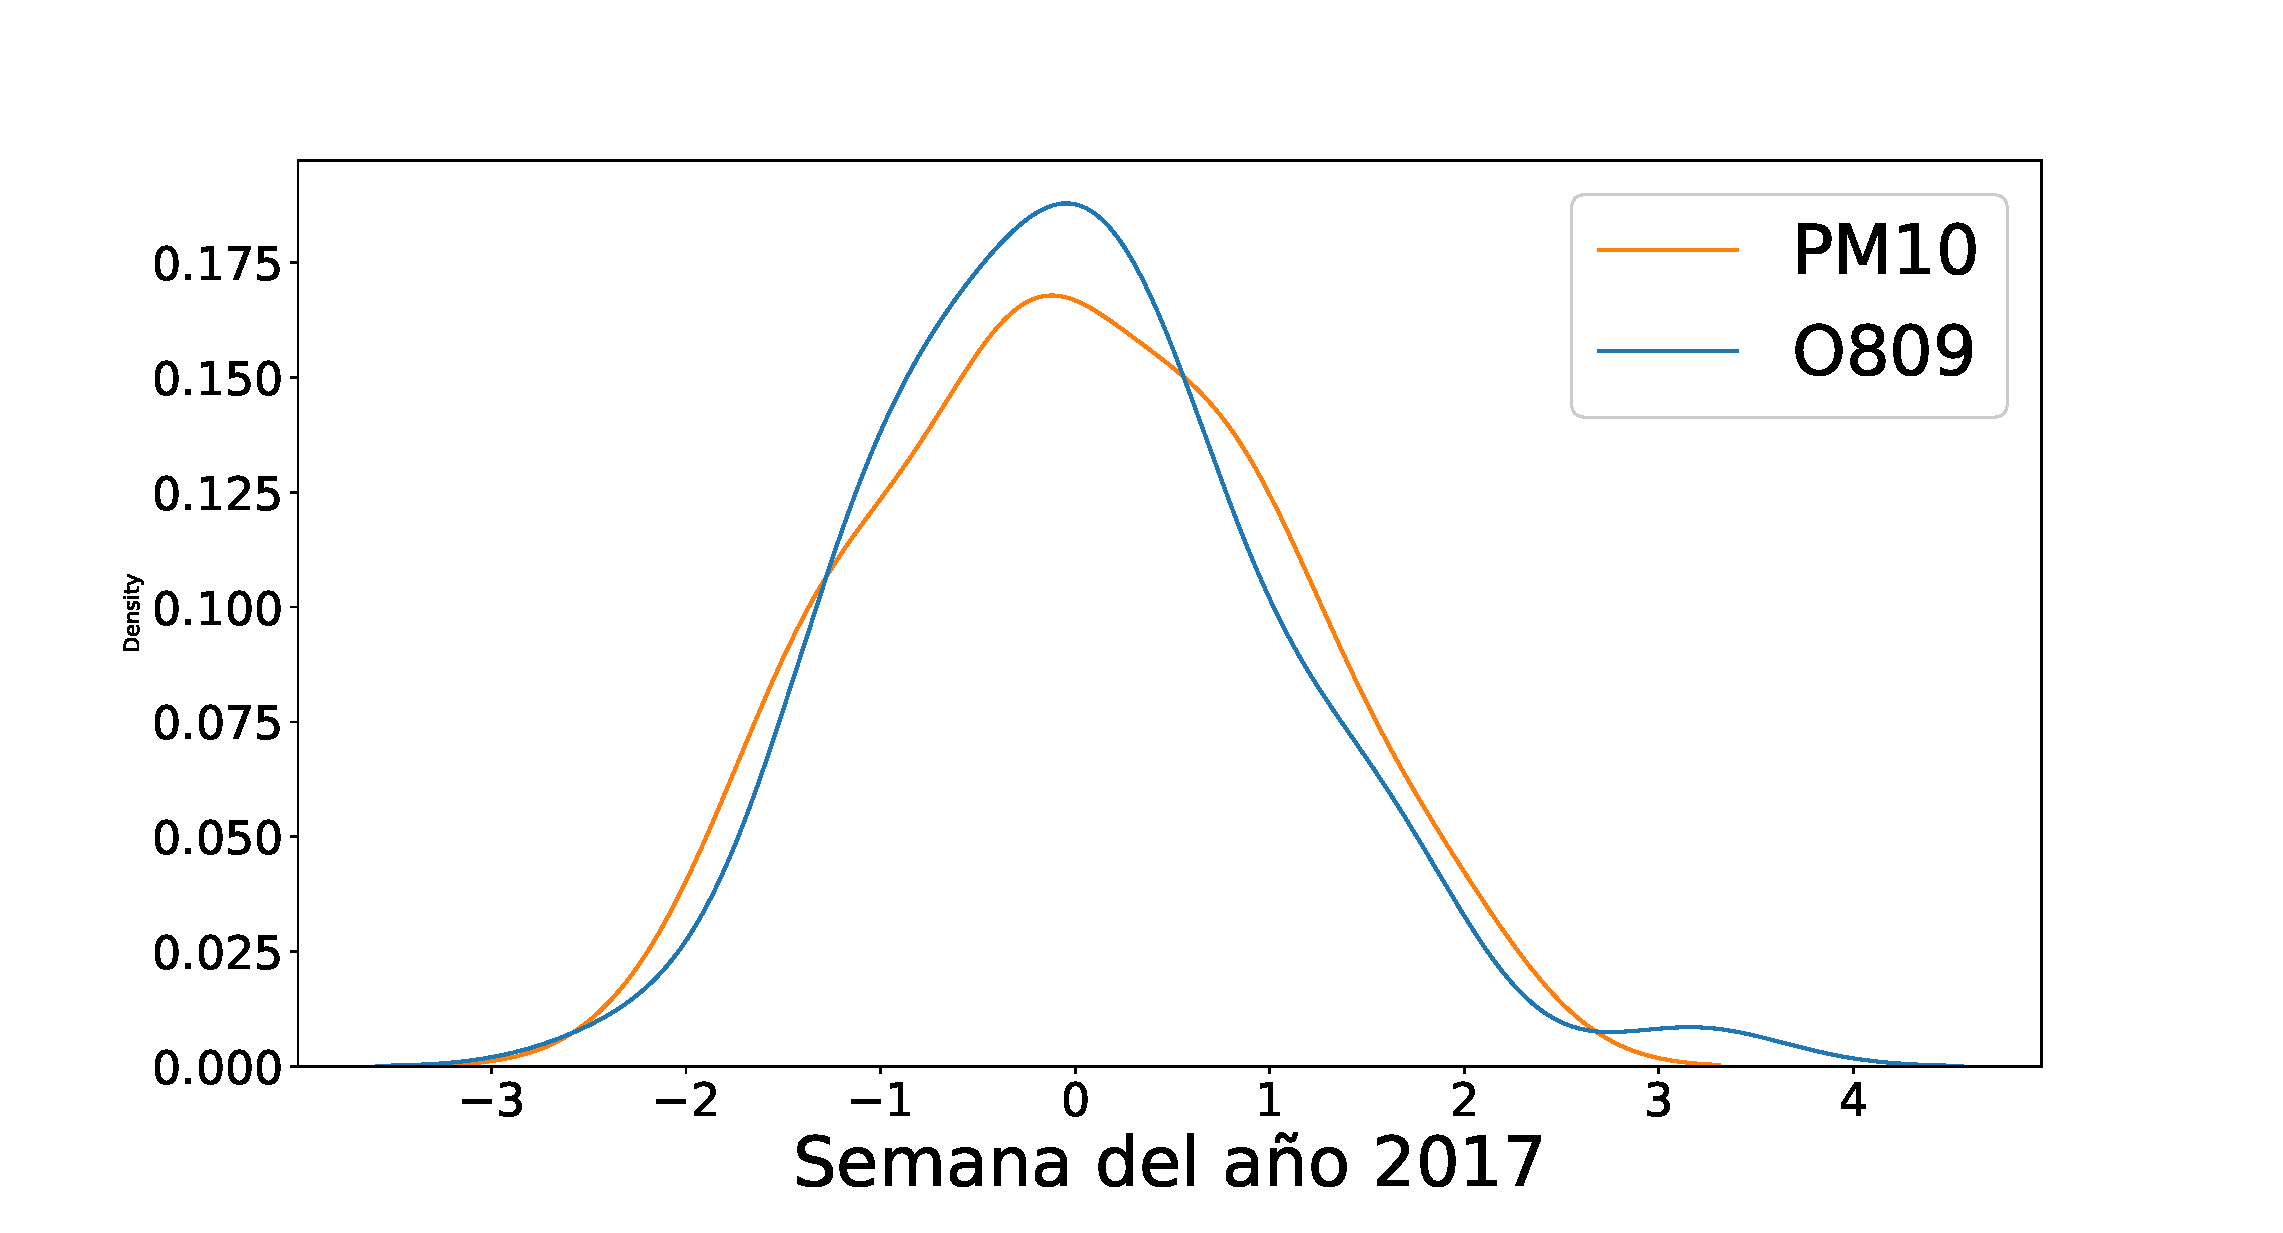
\includegraphics[trim=60 0 0 0,clip,width=0.9\textwidth]{PM10_O809_2017.eps}
   \end{center}
    \caption{Evolución de los niveles de PM10 y el número de egresos diagnosticados con la CIE O809 en el 2017.}
    \label{serie_de_tiempo_2017_PM10}
\end{figure}

\begin{figure}[h!]
\setcounter{figure}{2} % por culpa de sciposter
\captionsetup{type=figure} % por culpa de sciposter
\begin{center}
   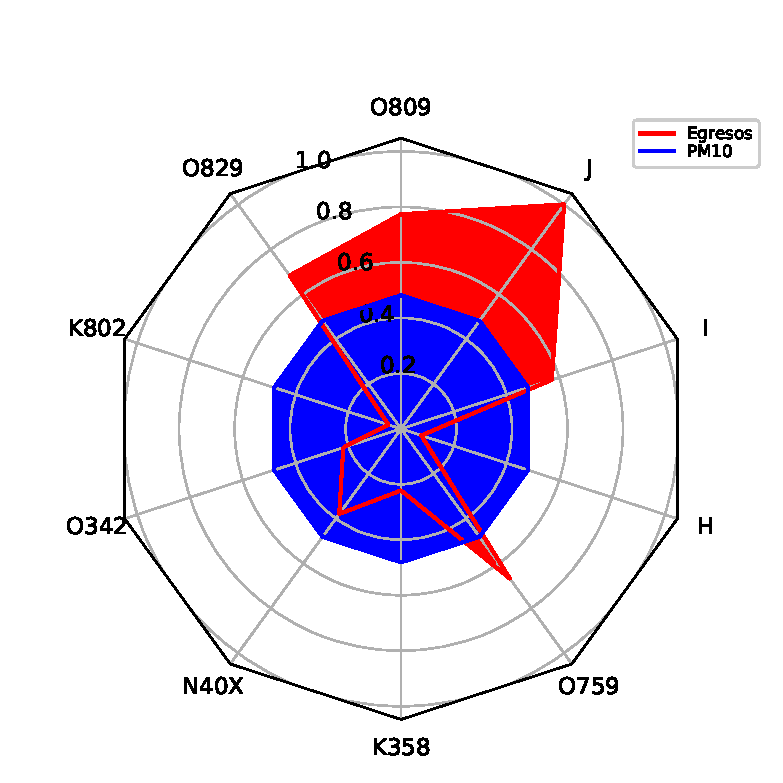
\includegraphics[trim=0 0 0 39,clip,width=0.8\textwidth]{spiderweb_PM10_2018_1.eps}
   \end{center}
    \caption{Nivel del contaminante PM10 y egresos por CIE en la semana 1 del año 2018.}
    \label{grafico_de_telaraña}
\end{figure}

\section{Experimentos}
$\rho$ = Coeficiente de correlación de Pearson

$\epsilon$ = RMSE para medir el error

\begin{table}[hbt!]
\centering
\captionsetup{type=table}
\setcounter{table}{1}
\caption{Resultados obtenidos para el año 2017. La tabla de la derecha muestra los resultados para PM10, y la tabla de la izquierda muestra para los resultados para PM2.5.}
\label{tab:Resultados obtenidos 2017}
\begin{adjustbox}{width=1\textwidth}
\begin{tabular}{|c|c|c|c|c|}
	\hline
	CIE & $\rho$ & $R^2$ & Valor $p$ & $\epsilon$\\
	\hline
	O809 & -0.275 & 0.061 & 0.121 & 0.239 \\
	\hline
	O829 & 0.100 & 0.091 & 0.055 & 0.287 \\
	\hline
	O759 & -0.085 & 0.116 & 0.029 & 0.294 \\
	\hline
	O069 & -0.247 & 0.070 & 0.094 & 0.222 \\
	\hline
	K802 & 0.044 & 0.005 & 0.658 & 0.282 \\
	\hline
\end{tabular}
\hspace{0.5cm}
\begin{tabular}{|c|c|c|c|c|}
	\hline
	$\rho$ & $R^2$ & Valor $p$ & $\epsilon$\\
	\hline
	-0.093 & 0.011 & 0.511 & 0.256 \\
	\hline
	0.014 & 0.021 & 0.371 & 0.253 \\
	\hline
	-0.172 & 0.113 & 0.032 & 0.278 \\
	\hline
	-0.350 & 0.112 & 0.033 & 0.208 \\
	\hline
	0.006 & 0.005 & 0.667 & 0.285 \\
	\hline
\end{tabular}
\end{adjustbox}
\end{table}

\begin{table}[hbt!]
\centering
\captionsetup{type=table}
\setcounter{table}{2}
\caption{Resultados obtenidos para el año 2018. La tabla de la derecha muestra los resultados para PM10, y la tabla de la izquierda muestra para los resultados para PM2.5.}
\label{tab:Resultados obtenidos 2018}
\begin{adjustbox}{width=1\textwidth}
\begin{tabular}{|c|c|c|c|c|}
	\hline
	CIE & $\rho$ & $R^2$ & Valor $p$ & $\epsilon$\\
	\hline
	O809 & -0.271 & 0.015 & 0.440 & 0.275 \\
	\hline
	O829 & 0.282 & 0.069 & 0.098 & 0.249 \\
	\hline
	K802 & 0.277 & 0.084 & 0.066 & 0.152 \\
	\hline
	O342 & -0.401 & 0.100 & 0.044 & 0.248 \\
	\hline
	N40X & -0.009 & 0.000 & 0.964 & 0.243 \\
	\hline
\end{tabular}
\hspace{0.5cm}
\begin{tabular}{|c|c|c|c|c|}
	\hline
	$\rho$ & $R^2$ & Valor $p$ & $\epsilon$\\
	\hline
	-0.354 & 0.057 & 0.133 & 0.259 \\
	\hline
	0.225 & 0.046 & 0.177 & 0.256 \\
	\hline
	0.273 & 0.089 & 0.058 & 0.159 \\
	\hline
	-0.443 & 0.149 & 0.013 & 0.245 \\
	\hline
	-0.074 & 0.001 & 0.842 & 0.241 \\
	\hline
\end{tabular}
\end{adjustbox}
\end{table}


\section{Conclusiones}
En las series de tiempo se observa que la cantidad de egresos de la mayoría de las CIE estudiadas presentan
una línea de evolución similar al contaminante PM10.
Además, se observó que para el estudio de las relaciones entre los contaminantes y las CIE se obtuvieron mejores resultados con los modelos de regresión lineal múltiple frente a los modelos de regresión lineal simple.


\subsection*{Agradecimientos}

Se cuenta con el financiamiento del programa PAICYT-UANL bajo las claves CE1421-20 y CE1842-21. El póster se preparó con \url{https://www.overleaf.com/}.

{\tiny \bibliography{MiBiblio}}
\bibliographystyle{plainnat}
\begin{table}
	\centering
	\begin{tabular}{c c}
		
\includegraphics[width=0.39\textwidth]{qr-code-poster.png} & 
\includegraphics[width=0.39\textwidth]{qr-code.png} \\
		Póster en línea & Repositorio en línea
	\end{tabular}
\end{table}
    
\end{multicols}

\end{document}